\documentclass[11pt,a4paper]{extarticle}

\usepackage[top=1.5in]{geometry}
\usepackage{amsmath}
\usepackage{graphicx}
\usepackage{titling}
\usepackage{changepage}
\usepackage{multicol}
\usepackage{listings}
\graphicspath{{images/}}

\setlength{\droptitle}{-10em}

\title{\textbf{Graph Theory \& Algorithms}}
\date{23 December 2017}
\author{Aniket Pandey}

\begin{document}
\maketitle

\section{Introduction}
Graph Theory is the study of Graphs, the mathematical objects modelling the pairwise relation of Vertices(also called nodes) and Edges where two nodes are connected by edges. A graph can be directed or undirected, cyclic or acyclic, linear or weighted etc. 

Graph Theoretical concepts are widely used to study and model various applications, in different areas. For example, in Computer Science, problems like travelling salesman problem, the shortest spanning tree in a weighted graph and in Mathematics like hamiltonian graphs and Fermat's Little Theorem \& Nielson-Schreier Theorem. 

\section{Notations}
\subsection{Big-O Notation}
Big-O Notations are used in mathematics to characterize functions according to their growth rate. In Graph Theory, efficiency of an algorithm is measured in terms of the input length $n$ as $n\rightarrow \infty $.\par Formal definition would be\\If $f:N\rightarrow N$ and $g:N\rightarrow N$ are two functions, then $f=$O$(g)$ if and only if $f(n)<c \cdot g(n)$ for a constant $c$ as $n\rightarrow\infty$.
\subsection{Other Notations}
There are a few more notations which complement Big-O Notation. I will give a brief information about these.\par
For functions $f$ \& $g$ from $N$ to $N$

\begin{align}
f =&\:\Omega(g)\quad  \textrm{if} \,\,  g=O(f)\\
f =&\:\Theta(g)\quad \textrm{if} \,\,  f=O(g) \,\, \& \,\, g=O(f)\\
f =&\:o(g)\:\,\quad \textrm{if there exists }\varepsilon \textrm{ such that} \,\, f(n)<\varepsilon\cdot g(n) \\
f =&\:\omega(g)\quad \:\textrm{if} \,\,  g=o(f)
\end{align}

\section{Terminologies}
Here are a few basic terminologies that are used to represent navigation through the Graph. \\
\begin{adjustwidth}{1.5em}{0pt}
\begin{description}
\item [Walk] A walk is any route through a graph from vertex to vertex along edges. A walk can end on the same vertex on which it began or on a different vertex. A walk can travel over any edge and any vertex any number of times.
\item [Path] A path is a walk that does not include any vertex twice, except that its first vertex might be the same as its last.
\item [Trail] A trail is a walk that does not pass over the same edge twice. A trail might visit the same vertex twice, but only if it comes and goes from a different edge each time.
\item [Cycle] A cycle is a path that begins and ends on the same vertex.	
\end{description}
\end{adjustwidth}

\section{Data Structures used in Graphs}
\subsection{Adjacency List}
An Adjacency List is a collection of unordered lists used to represent a finite graph. Each list describes the set of neighbors of a vertex in the graph.
\begin{center}
	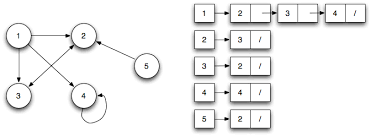
\includegraphics[width=8cm, height=3cm]{list}
\end{center} 

\subsection{Adjacency Matrix}
An Adjacency Matrix is a square matrix used to represent a finite graph. The elements of the matrix indicate whether pairs of vertices are adjacent or not in the graph.
\begin{center}
	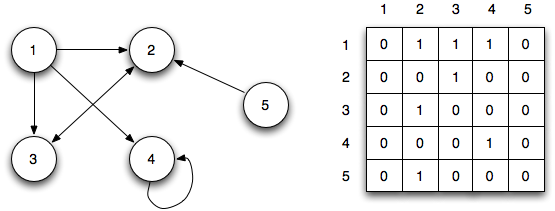
\includegraphics[width=8cm, height=3cm]{matrix}
\end{center}
 
\subsection{Stacks and Queues} 
Stacks and Queues are dynamic sets in which the element removed from the set by the \textit{delete} operation is prespecified. In a Stack, the element deleted from the set is the one inserted most recently, while in a Queue, the element that is to be deleted is the element which has been in the Queue for the longest time. \\

A \textbf{Stack} is a container of objects that are inserted and removed according to the last-in first-out (LIFO) principle. In the pushdown stacks only two operations are allowed: push the item into the stack, and pop the item out of the stack.

A \textbf{Queue} is a container of objects that are inserted and removed according to the first-in first-out (FIFO) principle. In the queue only two operations are allowed, enqueue and dequeue. Enqueue means to insert an item into the back of the queue, dequeue means removing the front item.
\newpage
\begin{multicols}{2}

\begin{center}
	\textbf{STACK}
\end{center}

\lstinputlisting[language=Python, showstringspaces=false]{code/stack.py}

\columnbreak

\begin{center}
	\textbf{QUEUE}
\end{center}

\lstinputlisting[language=Python, showstringspaces=false]{code/queue.py}

\end{multicols}

\section{BFS and DFS}
\subsection{Breadth First Search}
Breadth First Search (or BFS) is a graph traversal algorithm through which we can determine the shortest path from a source node $V$ to any other node in the graph, which is visitable from $V$. BFS works by starting from the source node, then visits all its neighbours, assignes them the value $1$ (distance from $V$). It continues the process by visiting the neighbours of the current node which have not already been visited, assignes them the respective value.

Now the question is, how do we keep track of all visited nodes. Well, for that we use a \textit{boolean array} and a \textit{queue} for storing the status of each node and for storing a node's unvisited neighbours respectively. 

Here is a simple pseudocode of BFS. 

\begin{adjustwidth}{2.5em}{0pt}
\lstinputlisting[language=Python, showstringspaces=false]{code/bfs.py}
\end{adjustwidth}

\subparagraph{Explanation and Analysis}
In the beginning I have declared an empty set $visited$, and enqueued the source node $S$. Then as long as queue $Q$ is not empty (there are unvisited nodes), we'll dequeue it and check all its neighbours, if they have not been visited, enqueue them and mark them as visited. This process will continue till every node is in the visited array. We can further run a test in the boolean array to check if there is a node which cannot be visited from the source node.

For example, in the image shown below, the node 7 cannot be visited from the source node 3.

\begin{center}
	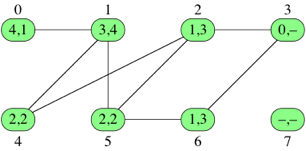
\includegraphics[width=8cm, height=3cm]{bfs}
\end{center}

\subparagraph{Time Complexity}
BFS loops through each Vertex and Edge to check the visited condition. So the complexity is,

\begin{align}
O(V,E) =& \,\,\,O(V+E)
\end{align}

\subsection{Depth First Search}

Depth First Search (or DFS) is a recursive Graph traversal algorithm using which we can determine the minimum spanning tree, presence of cycles and to check if the graph is bipartite. DFS works on the principle of backtracking, that is, it goes down a path, maintaining visited nodes in a \textit{stack} this time. When it can't find another unvisited node, it backtracks its path to the nearest node which has an unvisited neighbour. It continues this process until it lands back to the source node, implying that the traversal is complete.


\begin{adjustwidth}{2.5em}{0pt}
\lstinputlisting[language=Python, showstringspaces=false]{code/dfs.py}
\end{adjustwidth}

\subparagraph{Explanation and Analysis}
Apart from Graph and source node, the \textit{dfs} function also takes as an input an empty $stack$ which is used to keep track of visited chain of nodes, that is, we keep pushing onto the stack the nodes that have been visited, popping them once the recursion is complete. Then the part which checks for unvisited node is same as that in \textit{bfs}, only difference being we call dfs at every iteration.

\subparagraph{Time Complexity}
Same as that of BFS, the complexity of DFS is $O(V+E)$

\section{Single Source, Shortest Path}
Till now, both algorithms relied on the fact that the weight of each edge is unity. What if the weights were any integer (even negative), in that case, the algorithms discussed above will not work. For instance in the images shown below

\begin{multicols}{2}

\begin{center}
	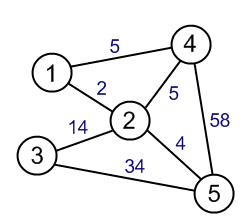
\includegraphics[width=5cm, height=3cm]{shortest}
\end{center}
Here, the direct path between 4 and 5 (58) is not the shortest one. 4-2-5 will be much shorter.

\columnbreak

\begin{center}
	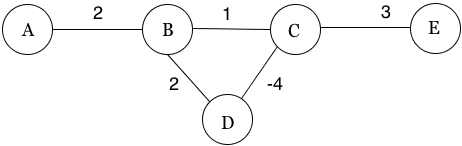
\includegraphics[width=6cm, height=3cm]{negative}
\end{center}

Here, the cycle $BCD$ has negative length (-1) implying the cycle has infinite negative weight.

\end{multicols}

To alleviate this issue, I'll discuss two algorithms, namely \textit{Dijkstra's Algorithm} \& \textit{Bellman-Ford Algorithm}

\subsection{Dijkstra's Algorithm}
Dijkstra’s algorithm finds a shortest path tree from a single source node, by building a set of nodes that have minimum distance from the source. The graph will have random connected nodes denoted by $u$ and $v$ and the weight of their edge will be $len(u,v)$. Purpose is to find the shortest path of every node from a given source node $s$.

\begin{adjustwidth}{2.5em}{0pt}
\lstinputlisting[language=Python, showstringspaces=false]{code/dijkstra.py}
\end{adjustwidth}

\subparagraph{Explanation and Analysis}
Dijkstra starts off by declaring an array \textit{dist} to store updated shortest distance of a node from the source. Clearly, $len(v,v) = 0$ and for every other node $u$, $dist[u] = \infty$. Now, we select the node which has the least distance from source (say $v$) and check if for a node $u$ $dist[v] + len(u,v) < dist[u]$. If so, then we update the value of $dist[u]$. This process continues till the no more updates can be done (Shortest paths have been found)

\subparagraph{Time Complexity}
The code which evaluates vertex $v$ for which $dist[v]$ is minimum can be a binary search of complexity $O(logV)$. For every node $v$, there are $v-1$ nodes and hence, $v-1$ possible edges (routes). So the complexity for Dijkstra is,

\begin{align}
O(V,E) =& \,\,\,O(V) + O((E-1)logV) + O(c)\\
	   =& \,\,\,O(Elog(V))
\end{align}

\subsection{Bellman-Ford Algorithm}
The Bellman-Ford is another algorithm which calculates the shortest paths from a single source. It is slower than Dijkstra, but for appropriate reasons as it also takes into account negative weights. If we put a Graph with negative edge cycles into Dijkstra, it will ignore those cycles and give wrong results.

\begin{adjustwidth}{2.5em}{0pt}
\lstinputlisting[language=Python, showstringspaces=false]{code/bell.py}
\end{adjustwidth}

\subparagraph{Explanation and Analysis}
Bellman-Ford works by overestimating the edge lengths of every node, assuming it to be a very large number. $node.prev = nil$ specifies the pointer to previous node which in this case has not yet been initialized. This algorithm relaxes the shortest path of each node by iterating over every possible edge, checks if $dist[v] > dist[u] + len(u,v)$ for adjacent nodes $(u,v)$ and if so, replaces the value of $dist[v]$. 

It has been proved that this iteration for $|V|$ times will make sure every shortest path is computed. Now, for the presence of any negative weight cycles, the last iteration again checks for triangular inequality for every pair $(u,v)$ in the Edge set. If it finds one, reports it as a negative weight cycle. 


\subparagraph{Time Complexity}
For various relaxations, Bellman-Ford check $|E|$ edges for every node in $|V|$. So the time complexity is,

\begin{align}
O(V,E) =& \,\,\,O(V) + O(V.E) + O(E) + O(c)\\
	   =& \,\,\,O(V.E)
\end{align}

\end{document}
